\chapter{Linear Regression Models} % Main appendix title

\label{Appendix_LinearRegression}


\section{Plant species - spectral species}

\subsection{Results over all test sites}

\begin{table}[ht]
\centering
\caption{Summary of linear regression model predicting plant species richness from spectral species richness over all test sites}
\begin{tabular}{lcccc}
\hline
\textbf{Predictor} & \textbf{Estimate} & \textbf{Std. Error} & \textbf{t value} & \textbf{Pr($>$$|$t$|$)} \\
\hline
Intercept & 57.2577 & 18.1108 & 3.162 & \textbf{0.00905**} \\
Unique Spectral Species & 0.5489 & 0.6323 & 0.868 & 0.40390 \\
\hline
\multicolumn{5}{l}{\textit{Residual standard error:} 33.38 on 11 degrees of freedom} \\
\multicolumn{5}{l}{\textit{Multiple R-squared:} 0.06411 \quad \textit{Adjusted R-squared:} -0.02097} \\
\multicolumn{5}{l}{\textit{F-statistic:} 0.7535 on 1 and 11 DF, \quad \textit{p-value:} 0.4039} \\
\hline
\end{tabular}
\label{tab:lm_plantspecies_spectral}
\end{table}

\begin{figure}[H]
    \centering
    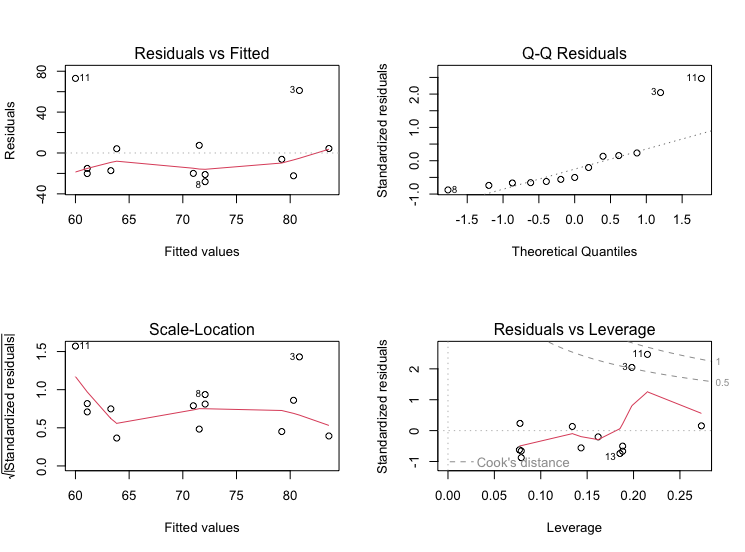
\includegraphics[width=0.9\textwidth]{Figures/Appendix/LRM_Plots/all_model_plant_species_lm.png} % Replace with your actual image path
    \caption{Residual plots for the linear regression model to predict pant species numbers from spectral species over all plots. Clear outliers are detectable in the residual vs fitted and the Q-Q residual plot (3 and 11)}
    \label{fig:all_model_plant_species_lm}
\end{figure}

\subsection{Results for Group C/D}
\begin{table}[ht]
\centering
\caption{Summary of linear regression model predicting plant species richness from spectral species richness for Group C/D}
\begin{tabular}{lcccc}
\hline
\textbf{Predictor} & \textbf{Estimate} & \textbf{Std. Error} & \textbf{t value} & \textbf{Pr($>$$|$t$|$)} \\
\hline
Intercept & 62.2493 & 25.3566 & 2.455 & \textbf{0.0396*} \\
Unique Spectral Species & 0.3982 & 0.8102 & 0.491 & 0.6363 \\
\hline
\multicolumn{5}{l}{\textit{Residual standard error:} 38.28 on 8 degrees of freedom} \\
\multicolumn{5}{l}{\textit{Multiple R-squared:} 0.02931 \quad \textit{Adjusted R-squared:} -0.09203} \\
\multicolumn{5}{l}{\textit{F-statistic:} 0.2416 on 1 and 8 DF, \quad \textit{p-value:} 0.6363} \\
\hline
\end{tabular}
\label{tab:lm_plantspecies_spectral_group_cd}
\end{table}

\begin{figure}[H]
    \centering
    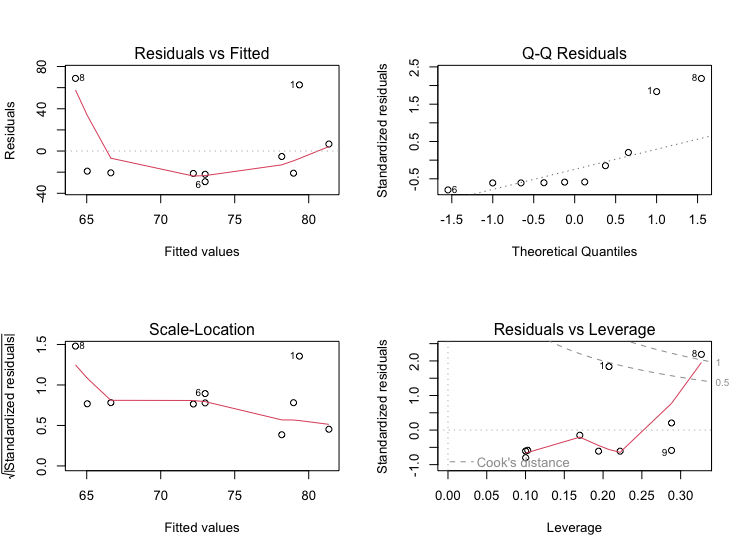
\includegraphics[width=0.9\textwidth]{Figures/Appendix/LRM_Plots/group_c_d_model_plant_species_lm.png} % Replace with your actual image path
    \caption{Residual plots for the linear regression model to predict plant species numbers from spectral species in group C/D. Clear outliers are detectable in the residual vs fitted and the Q-Q residual plot (1 and 8)}
    \label{fig:group_c_d_model_plant_species_lm}
\end{figure}

\subsection{Results for Group E}
\begin{table}[ht]
\centering
\caption{Summary of linear regression model predicting plant species richness from spectral species richness for Group E}
\begin{tabular}{lcccc}
\hline
\textbf{Predictor} & \textbf{Estimate} & \textbf{Std. Error} & \textbf{t value} & \textbf{Pr($>$$|$t$|$)} \\
\hline
Intercept & 36.6100 & 16.3602 & 2.238 &  0.268 \\
Unique Spectral Species & 1.7371 & 0.9613 & 1.807 & 0.322 \\
\hline
\multicolumn{5}{l}{\textit{Residual standard error:} 13.39 on 1 degrees of freedom} \\
\multicolumn{5}{l}{\textit{Multiple R-squared:} 0.7656 \quad \textit{Adjusted R-squared:} 0.5311} \\
\multicolumn{5}{l}{\textit{F-statistic:} 3.266 on 1 and 1 DF, \quad \textit{p-value:} 0.3218} \\
\hline
\end{tabular}
\label{tab:lm_plantspecies_spectral_group_e}
\end{table}

\begin{figure}[H]
    \centering
    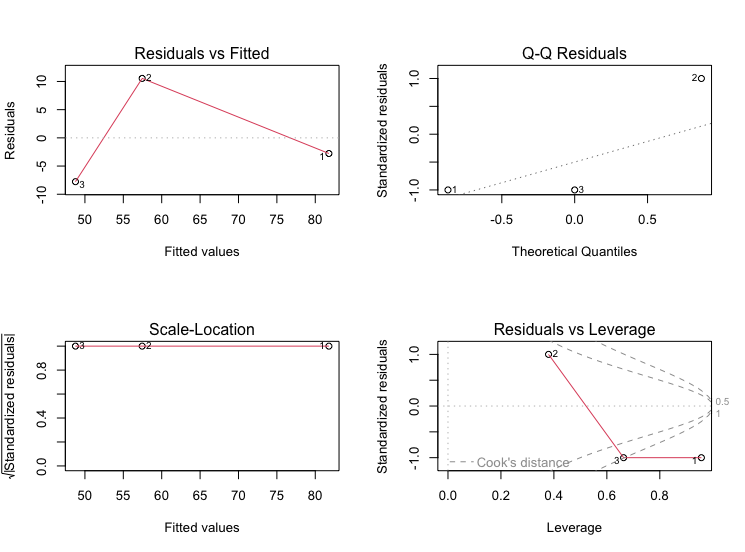
\includegraphics[width=0.9\textwidth]{Figures/Appendix/LRM_Plots/group_e_model_plant_species_lm.png} % Replace with your actual image path
    \caption{Residual plots for the linear regression model to predict plant species numbers from spectral species in group E. Since there are so few data points the the results don't hold any value.}
    \label{fig:group_e_model_plant_species_lm}
\end{figure}


\section{Plant communities - spectral species}
\subsection{Results over all test sites}
\begin{table}[ht]
\centering
\caption{Summary of linear regression model predicting plant community richness from spectral species richness over all test sites}
\begin{tabular}{lcccc}
\hline
\textbf{Predictor} & \textbf{Estimate} & \textbf{Std. Error} & \textbf{t value} & \textbf{Pr($>$$|$t$|$)} \\
\hline
Intercept & 9.08876 & 2.53324 & 3.588 & \textbf{0.00426**} \\
Unique Spectral Species & -0.02236 & 0.08845 & -0.253 & 0.80512 \\
\hline
\multicolumn{5}{l}{\textit{Residual standard error:} 4.669 on 11 degrees of freedom} \\
\multicolumn{5}{l}{\textit{Multiple R-squared:} 0.005774 \quad \textit{Adjusted R-squared:} -0.08461} \\
\multicolumn{5}{l}{\textit{F-statistic:} 0.06389 on 1 and 11 DF, \quad \textit{p-value:} 0.8051} \\
\hline
\end{tabular}
\label{tab:lm_plant_community_spectral}
\end{table}

\begin{figure}[H]
    \centering
    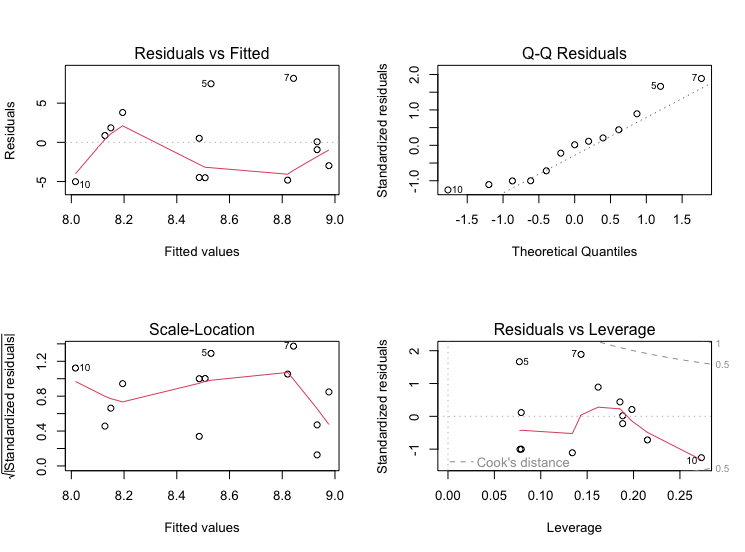
\includegraphics[width=0.9\textwidth]{Figures/Appendix/LRM_Plots/all_model_plant_communities_lm.png} % Replace with your actual image path
    \caption{Residual plots for the linear regression model to predict plant community numbers from spectral species over all plots.}
    \label{fig:all_model_plant_communities_lm}
\end{figure}

\subsection{Results for Group C/D}
\begin{table}[ht]
\centering
\caption{Summary of linear regression model predicting plant community richness from spectral species richness for Group C/D}
\begin{tabular}{lcccc}
\hline
\textbf{Predictor} & \textbf{Estimate} & \textbf{Std. Error} & \textbf{t value} & \textbf{Pr($>$$|$t$|$)} \\
\hline
Intercept & 11.00134 & 3.18381 & 3.455 & \textbf{0.00863**} \\
Unique Spectral Species & -0.05823 & 0.10173 & -0.572 & 0.58277 \\
\hline
\multicolumn{5}{l}{\textit{Residual standard error:} 4.807 on 8 degrees of freedom} \\
\multicolumn{5}{l}{\textit{Multiple R-squared:} 0.03935 \quad \textit{Adjusted R-squared:} -0.08074} \\
\multicolumn{5}{l}{\textit{F-statistic:} 0.3277 on 1 and 8 DF, \quad \textit{p-value:} 0.5828} \\
\hline
\end{tabular}
\label{tab:lm_plantspecies_spectral}
\end{table}

\begin{figure}[H]
    \centering
    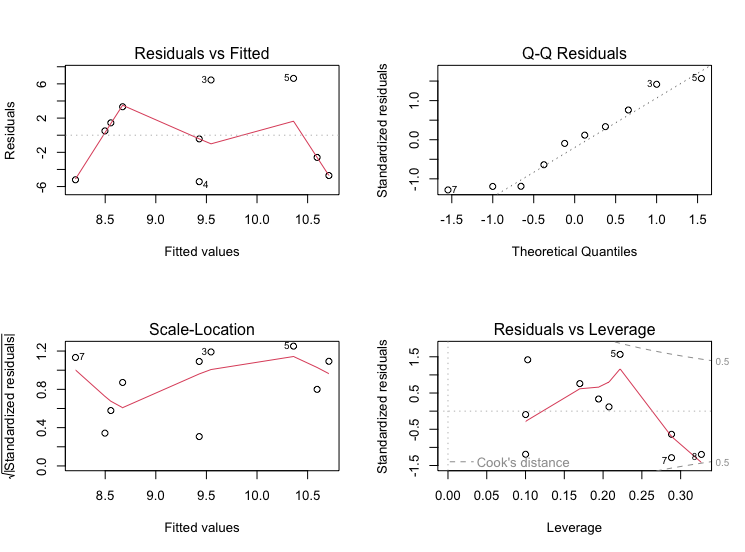
\includegraphics[width=0.9\textwidth]{Figures/Appendix/LRM_Plots/group_c_d_model_plant_communities_lm.png} % Replace with your actual image path
    \caption{Residual plots for the linear regression model to predict plant community numbers from spectral species in group C/D.}
    \label{fig:group_c_d_model_plant_communities_lm}
\end{figure}

\subsection{Results for Group E}
\begin{table}[ht]
\centering
\caption{Summary of linear regression model predicting plant community richness from spectral species richness for Group E}
\begin{tabular}{lcccc}
\hline
\textbf{Predictor} & \textbf{Estimate} & \textbf{Std. Error} & \textbf{t value} & \textbf{Pr($>$$|$t$|$)} \\
\hline
Intercept & 8.7595 & 3.5456 & 2.471 & 0.245 \\
Unique Spectral Species & -0.2062 & 0.2083 & -0.990 & 0.503 \\
\hline
\multicolumn{5}{l}{\textit{Residual standard error:} 2.902 on 1 degrees of freedom} \\
\multicolumn{5}{l}{\textit{Multiple R-squared:} 0.4948 \quad \textit{Adjusted R-squared:} -0.01031} \\
\multicolumn{5}{l}{\textit{F-statistic:} 0.9796 on 1 and 1 DF, \quad \textit{p-value:} 0.5033} \\
\hline
\end{tabular}
\label{tab:lm_plantspecies_spectral}
\end{table}

\begin{figure}[H]
    \centering
    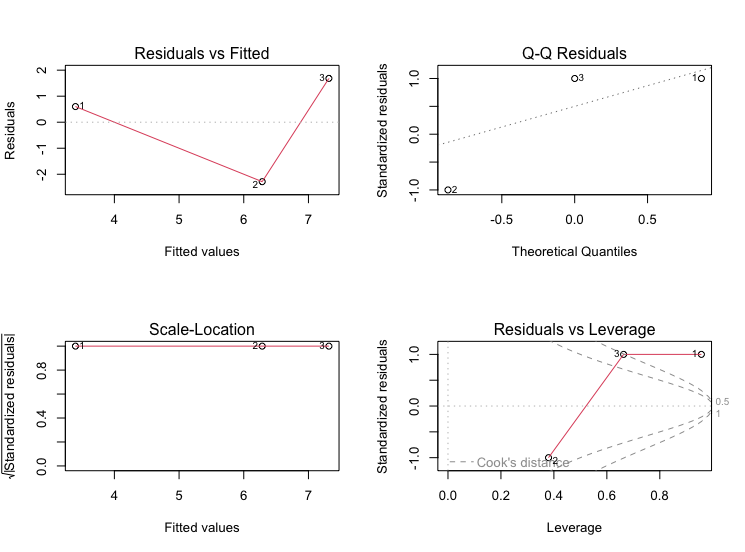
\includegraphics[width=0.9\textwidth]{Figures/Appendix/LRM_Plots/group_e_model_plant_communities_lm.png} % Replace with your actual image path
    \caption{Residual plots for the linear regression model to predict plant community numbers from spectral species in group E.}
    \label{fig:group_e_model_plant_communities_lm}
\end{figure}

\section{Habitat types - spectral species}
\begin{table}[ht]
\centering
\caption{Summary of linear regression model predicting habitat type richness from spectral species richness over all test sites}
\begin{tabular}{lcccc}
\hline
\textbf{Predictor} & \textbf{Estimate} & \textbf{Std. Error} & \textbf{t value} & \textbf{Pr($>$$|$t$|$)} \\
\hline
Intercept & 2.94635 & 0.86879 & 3.391 & \textbf{0.00602**} \\
Unique Spectral Species & 0.03030 & 0.03033 & 0.999 & 0.33925 \\
\hline
\multicolumn{5}{l}{\textit{Residual standard error:} 1.601 on 11 degrees of freedom} \\
\multicolumn{5}{l}{\textit{Multiple R-squared:} 0.08319 \quad \textit{Adjusted R-squared:} -0.0001603} \\
\multicolumn{5}{l}{\textit{F-statistic:} 0.9981 on 1 and 11 DF, \quad \textit{p-value:} 0.3392} \\
\hline
\end{tabular}
\label{tab:lm_habitat_type_spectral}
\end{table}

\begin{figure}[H]
    \centering
    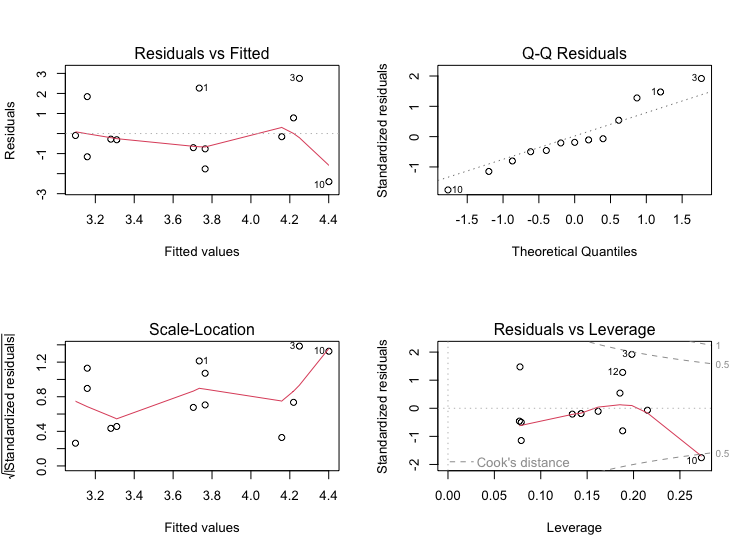
\includegraphics[width=0.9\textwidth]{Figures/Appendix/LRM_Plots/all_model_habitat_types_lm.png} % Replace with your actual image path
    \caption{Residual plots for the linear regression model to predict habitat type numbers from spectral species over all plots.}
    \label{fig:all_model_habitat_types_lm}
\end{figure}


\subsection{Results for Group C/D}
\begin{table}[ht]
\centering
\caption{Summary of linear regression model predicting habitat type richness from spectral species richness for Group C/D}
\begin{tabular}{lcccc}
\hline
\textbf{Predictor} & \textbf{Estimate} & \textbf{Std. Error} & \textbf{t value} & \textbf{Pr($>$$|$t$|$)} \\
\hline
Intercept & 3.17648 & 1.08058 & 2.940 & \textbf{0.0187*} \\
Unique Spectral Species & 0.01904 & 0.03453 & 0.551 & 0.5964 \\
\hline
\multicolumn{5}{l}{\textit{Residual standard error:} 1.631 on 8 degrees of freedom} \\
\multicolumn{5}{l}{\textit{Multiple R-squared:} 0.03661 \quad \textit{Adjusted R-squared:} -0.08381} \\
\multicolumn{5}{l}{\textit{F-statistic:} 0.304 on 1 and 8 DF, \quad \textit{p-value:} 0.5964} \\
\hline
\end{tabular}
\label{tab:lm_plantspecies_spectral}
\end{table}

\begin{figure}[H]
    \centering
    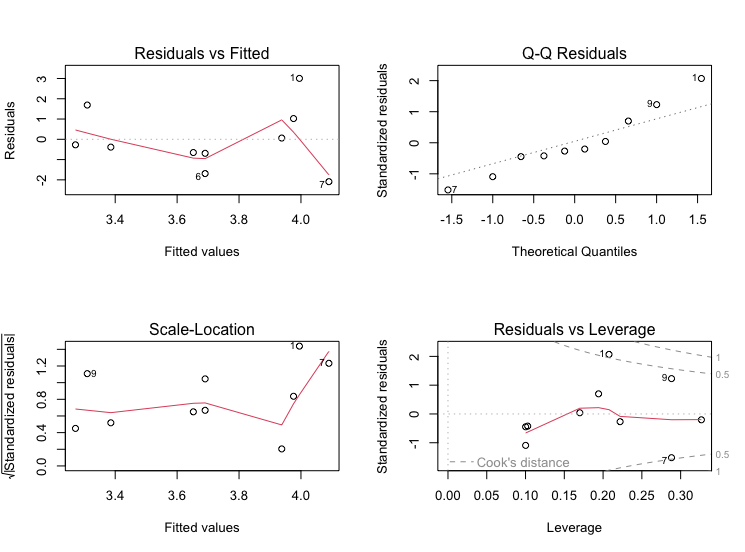
\includegraphics[width=0.9\textwidth]{Figures/Appendix/LRM_Plots/group_c_d_model_habitat_types_lm.png} % Replace with your actual image path
    \caption{Residual plots for the linear regression model to predict habitat type numbers from spectral species in group C/D.}
    \label{fig:group_c_d_model_habitat_types_lm}
\end{figure}

\subsection{Results for Group E}
\begin{table}[ht]
\centering
\caption{Summary of linear regression model predicting habitat type richness from spectral species richness for Group E}
\begin{tabular}{lcccc}
\hline
\textbf{Predictor} & \textbf{Estimate} & \textbf{Std. Error} & \textbf{t value} & \textbf{Pr($>$$|$t$|$)} \\
\hline
Intercept & 0.496564 & 0.050651 & 9.804 & 0.06471 \\
Unique Spectral Species & 0.211340 & 0.002976 & 71.014 & \textbf{0.00896**} \\
\hline
\multicolumn{5}{l}{\textit{Residual standard error:} 0.04145 on 1 degrees of freedom} \\
\multicolumn{5}{l}{\textit{Multiple R-squared:} 0.9998 \quad \textit{Adjusted R-squared:} 0.9996} \\
\multicolumn{5}{l}{\textit{F-statistic:} 5043 on 1 and 1 DF, \quad \textit{p-value:} 0.008964} \\
\hline
\end{tabular}
\label{tab:lm_plantspecies_spectral}
\end{table}

\begin{figure}[H]
    \centering
    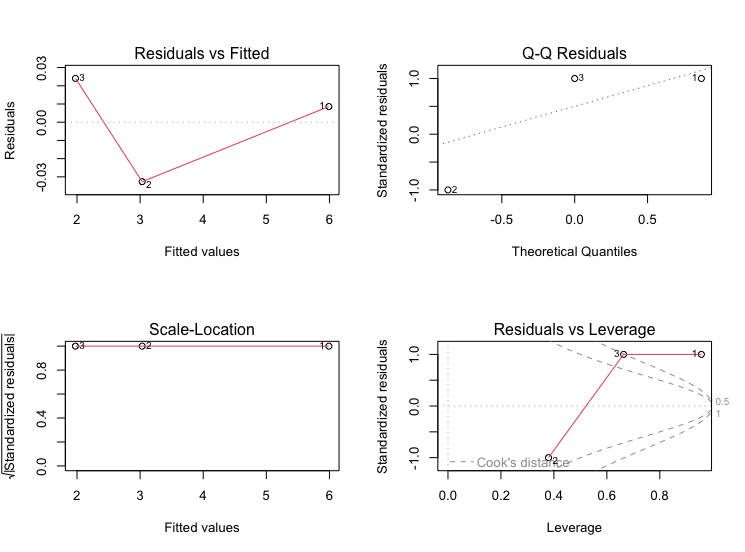
\includegraphics[width=0.9\textwidth]{Figures/Appendix/LRM_Plots/group_e_model_habitat_types_lm.png} % Replace with your actual image path
    \caption{Residual plots for the linear regression model to predict habitat type numbers from spectral species in group E.}
    \label{fig:group_e_model_habitat_types_lm}
\end{figure}